\begin{frame}{Forced oscillation}
Equation of motion:
\begin{equation} \label{eq:motion-general-forced}
	\ddot{\theta}+2 \gamma \dot{\theta} + \omega_0^2 \theta = f \, \cos(\omega t)
\end{equation}

\begin{description}
\item[$\gamma$] measure of dumping
\item[$\omega_0$] natural frequency
\item[$\omega$] angular frequency of the driving force
\item[$f$] measure of driving amplitude
\end{description}
\pause
Solution:
\begin{align}
\begin{split}
\theta(\omega) &=X(\omega)\cos(\omega t - \phi(\omega)) \\
X(\omega)&=\frac{f}{\sqrt{(\omega_0^2-\omega^2)^2+(2 \gamma \omega)^2}} \\
\tan \phi(\omega)&=\frac{2\gamma \omega}{\omega_0^2-\omega^2} \\
\end{split}
\end{align}
\end{frame}


\begin{frame}{Forced oscillation}
\begin{figure}[ht]
	\centering
	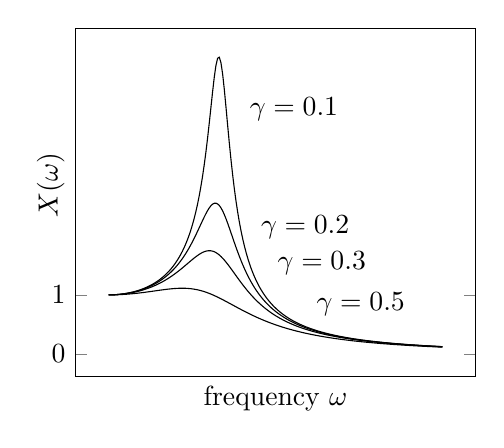
\begin{tikzpicture}[baseline]
	\begin{axis}[width=\textwidth*0.55,height=6cm,
	samples=200,domain=0:3,xlabel=frequency $\omega$, ylabel=$X(\omega)$,
	xtick=\empty,
	y label style={at={(axis description cs:-0.12,+0.55)},anchor=north},
	ytick={0,1}]
	\addplot[] {1/sqrt((1-x^2)^2+(2*x*0.1)^2)};
	\node at (axis cs:2.15,4.5) [anchor=north east] {$\gamma=0.1$};
	\addplot[] {1/sqrt((1-x^2)^2+(2*x*0.2)^2)};
	\node at (axis cs:2.25,2.5) [anchor=north east] {$\gamma=0.2$};
	\addplot[] {1/sqrt((1-x^2)^2+(2*x*0.3)^2)};
	\node at (axis cs:2.4,1.9) [anchor=north east] {$\gamma=0.3$};
	\addplot[] {1/sqrt((1-x^2)^2+(2*x*0.53)^2)};
	\node at (axis cs:2.75,1.2) [anchor=north east] {$\gamma=0.5$};
	\end{axis}
	\end{tikzpicture}%
	\hspace{0.2cm}
	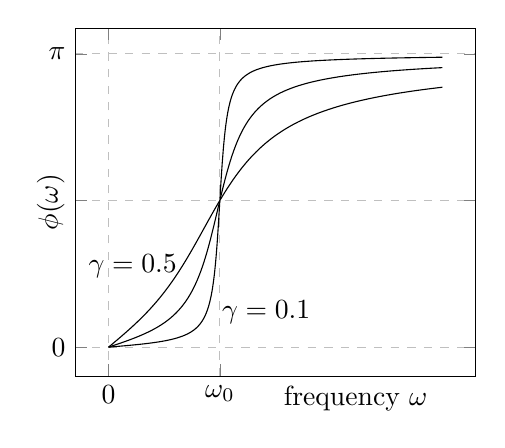
\begin{tikzpicture}[baseline]
	\begin{axis}[width=\textwidth*0.55,height=6cm,
	samples=200,domain=0:3,xlabel=frequency $\omega$, ylabel=$\phi(\omega)$,
	ytick={0,1.57, 3.14},
	yticklabels={$0$, \empty,$\pi$},
	xtick={0,1},
	xticklabels={$0$, $\omega_0$},
	x label style={at={(axis description cs:+0.7,-0.0)},anchor=north},
	y label style={at={(axis description cs:-0.12,+0.5)},anchor=north},
	grid style=dashed,
	xmajorgrids=true,ymajorgrids=true]
	\addplot[domain=0:1] {rad(atan(2*x*0.05/(1-x^2)))};
	\addplot[domain=1+0.001:3] {pi+rad(atan(2*x*0.05/(1-x^2)))};
	\node at (axis cs:1.9,0.6) [anchor=north east] {$\gamma=0.1$};
	\addplot[domain=0:1] {rad(atan(2*x*0.2/(1-x^2)))};
	\addplot[domain=1+0.001:3] {pi+rad(atan(2*x*0.2/(1-x^2)))};
	\addplot[domain=0:1] {rad(atan(2*x*0.5/(1-x^2)))};
	\addplot[domain=1+0.001:3] {pi+rad(atan(2*x*0.5/(1-x^2)))};
	\node at (axis cs:0.7,1.1) [anchor=north east] {$\gamma=0.5$};
	\end{axis}
	\end{tikzpicture}
	\caption{Dependence of \textit{amplitude} (on the left) and \textit{phase difference} (on the right) from frequency of the driving force}
	\label{fig:amplitude-frequency}
\end{figure}
\begin{columns}
\column{0.4\textwidth}
\begin{align*}
    \omega_{max} &= \sqrt{\omega_0^2-2\gamma^2}
\end{align*}
\column{0.6\textwidth}
\begin{align*}
    X_{max} \equiv X(\omega_{max}) &= \frac{f}{2\gamma\sqrt{\omega_0^2-\gamma^2}}
\end{align*}
\end{columns}

\end{frame}